Packet analysis for each of the simulations was performed using the Wireshark
tool. This tool can be run on the PC running Mininet, and configured to monitor
the loopback address for OpenFlow packets, as described in the "Start Wireshark"
section here \cite{mininetWS}, or can be run on one of the Mininet host nodes.

\subsection{Denial of Service Results}

The Denial of Service network is initiated using the command show in Figure
\ref{fig:images-dosMnCli}. The output of running this command shows that all of
the required nodes and links are successfully created.

\begin{figure}[H]
	\centering
	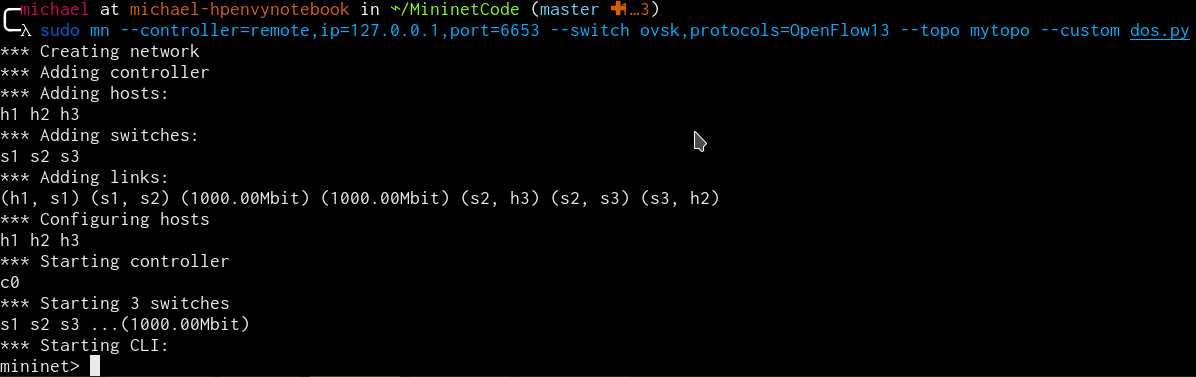
\includegraphics[width=0.8\textwidth]{images/dosMnCli}
	\caption{DoS Mininet CLI command output}
	\label{fig:images-dosMnCli}
\end{figure}

The Denial of Service topology was first verified within the Floodlight web
server. Figure \ref{fig:images-flDoS} displays the results of this:

\begin{figure}[H]
	\centering
	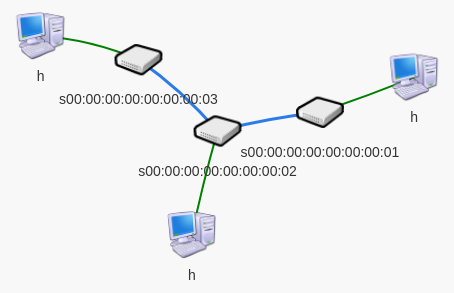
\includegraphics[width=0.8\textwidth]{images/flDoS}
	\caption{Denial of Service Floodlight Topology}
	\label{fig:images-flDoS}
\end{figure}

Once the network was deemed as correctly configure, the attack testing could
begin.

\subsubsection{SYN Flood}

The Wireshark packet analyser tool is run on the attacking host. The filter
option used to capture only the outgoing SYN packets from the host is
'tcp.flag.syn== 1'. This results in the packet capture in Figure
\ref{fig:images-synFloodDosWs}. The set "SYN" flag can be seen in the packet
information in the bottom of the window.

\begin{figure}[H]
	\centering
	\includegraphics[width=0.8\textwidth]{images/synFloodDosWs}
	\caption{Denial of Service SYN Flood Captured Packets}
	\label{fig:images-synFloodDosWs}
\end{figure}

The SYN flood was initiated as discussed, using the hping command listed in
section 3.1.1. Once the flooding attack had been running for a period of time,
the ping command is used on the user host node, showing multiple timeouts,
indicating a denial of service has occurred.

\begin{figure}[H]
	\centering
	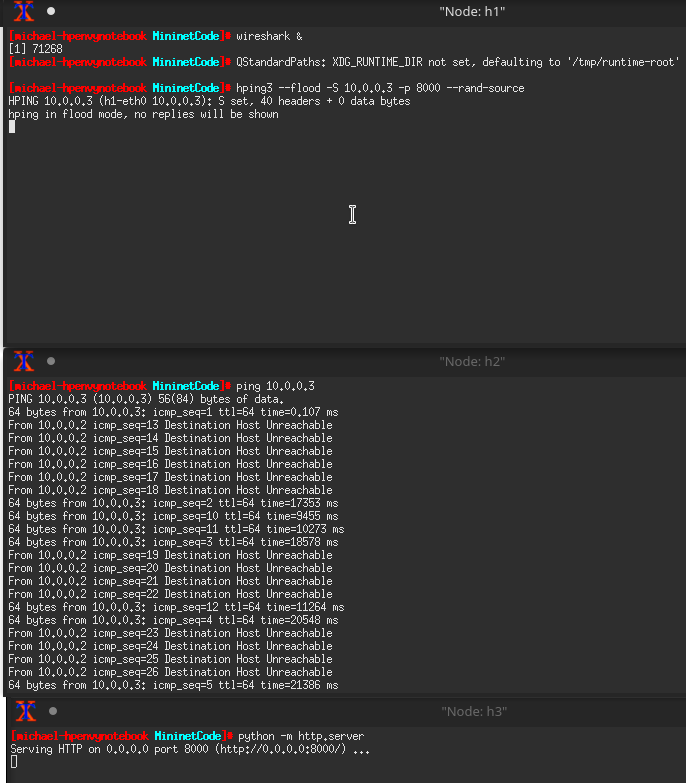
\includegraphics[width=0.8\textwidth]{images/synFloodResults}
	\caption{Terminal Output for the attacking node, target server, and user
	node}
	\label{fig:images-synFloodResults}
\end{figure}

The I/O graph output which can be viewed from the captured packets in Wireshark
shows the number of packets sent per second. There is a dip in the graph where
the number of sent packets drops to zero, which could account for the successful
ping connections from the user node.

\begin{figure}[H]
	\centering
	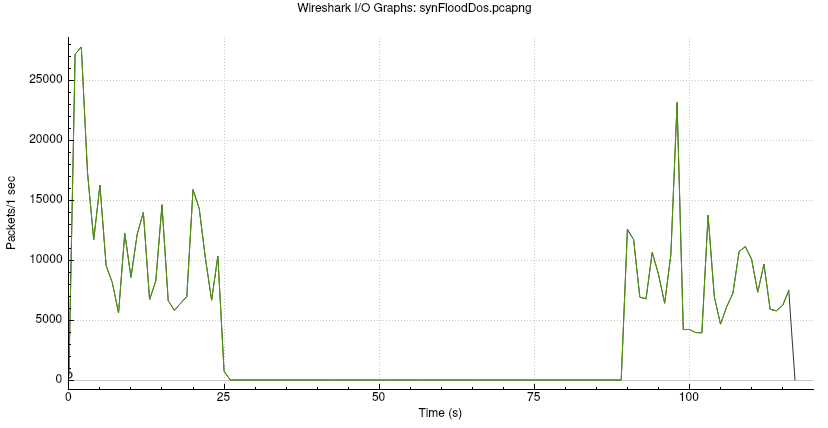
\includegraphics[width=0.8\textwidth]{images/synFloodDosIOGraph}
	\caption{Denial of Service SYN Attack I/O Graph}
	\label{fig:images-synFloodDosIOGraph}
\end{figure}

\subsubsection{ICMP Flood}

The Wireshark packet analyser tool is run on the attacking host. The filter
option used to capture only the outgoing ICMP packets from the host is
'icmp'. This results in the packet capture in Figure
\ref{fig:images-icmpFloodDosWs}.

\begin{figure}[H]
	\centering
	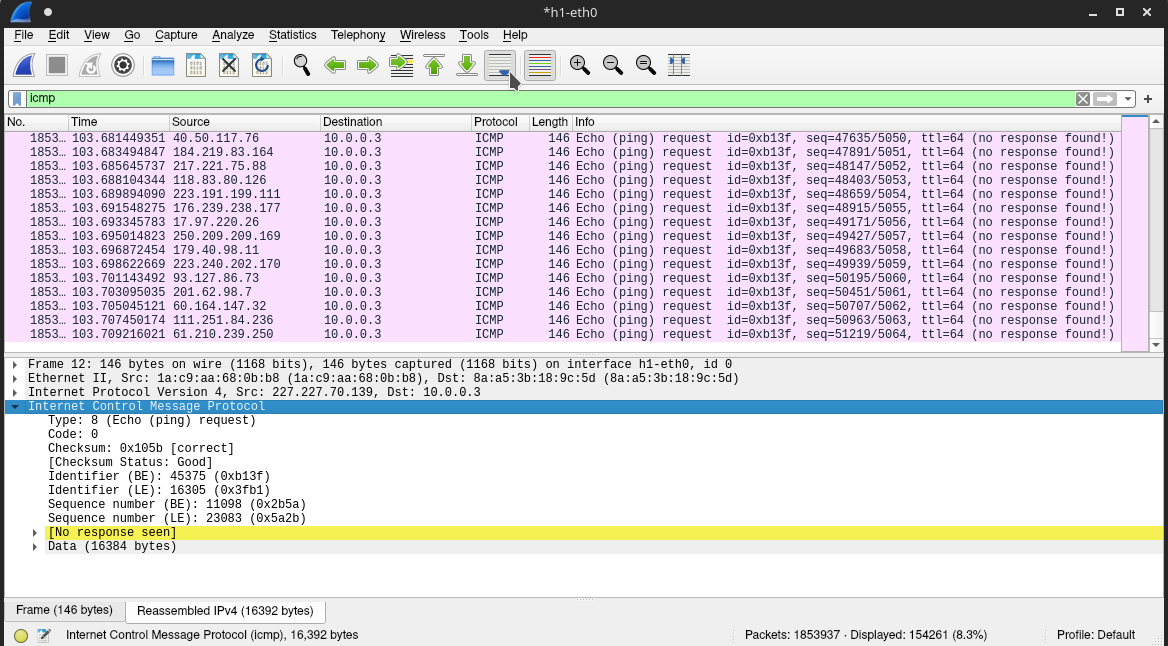
\includegraphics[width=0.8\textwidth]{images/icmpFloodDoSWs}
	\caption{Denial of Service ICMP Flood Captured Packets}
	\label{fig:images-icmpFloodDosWs}
\end{figure}

The ICMP flood was initiated as discussed, using the hping command listed in
section 3.1.2. Once the flooding attack had been running for a period of time,
the ping command is used on the user host node, showing 100\% packet loss,
indicating a denial of service has occurred.

\begin{figure}[H]
	\centering
	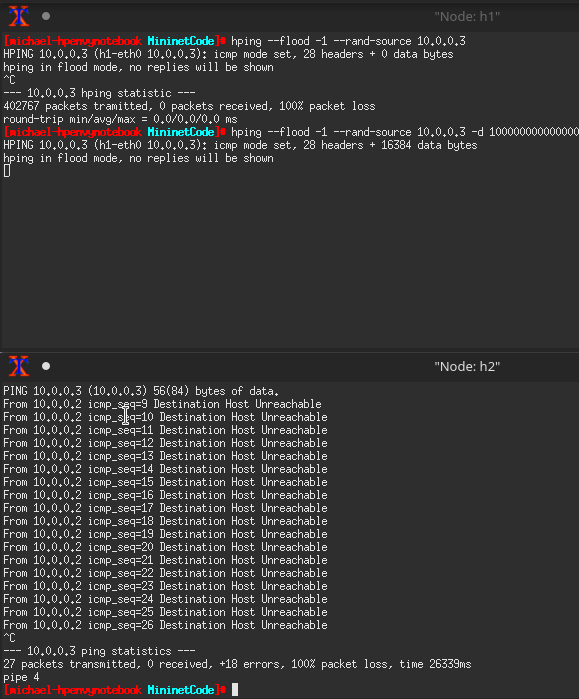
\includegraphics[width=0.8\textwidth]{images/IcmpFloodDosCli}
	\caption{Denial of Service ICMP Flood Output}
	\label{fig:images-icmpFloodDosCli}
\end{figure}

The I/O graph output which can be viewed from the captured packets in Wireshark
shows the number of packets sent per second. There are a number of dips in the
graph where the number of sent packets drops, at some points to zero, however,
this did not result in a successful ICMP echo response from the server.

\begin{figure}[H]
	\centering
	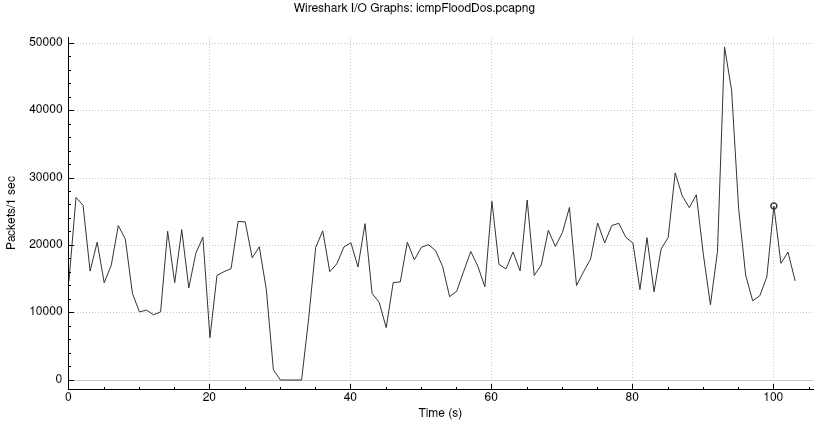
\includegraphics[width=0.8\textwidth]{images/icmpFloodDos}
	\caption{Denial of Service ICMP Attack I/O Graph}
	\label{fig:images-icmpFloodDosIOGraph}
\end{figure}

\subsubsection{Mitigation}

In order to utilise the benefits of SDN and the Floodlight controller, both of
these attacks could be mitigated using Network Access Control Lists. NACLs allow
for the blacklisting or whitelisting of different IP addresses for certain
protocols. For example, ICMP can be disabled for all nodes by specifying a deny
rule for the CIDR rage 0.0.0.0/0. In the case of the SYN Flood, which uses
random source IP addresses, whitelisting could be used to allow traffic from
nodes within the network, such as the user node, or for the case of the ICMP
Flood, which does not use spoofed IP addresses, the attack source IP address can
be blacklisted, as shown in Figure \ref{fig:images-icmpDosAcl}.

\begin{figure}[H]
	\centering
	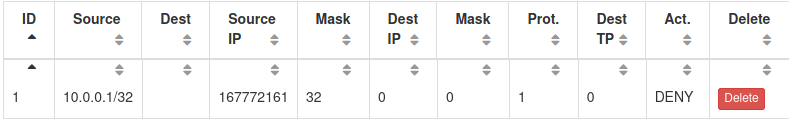
\includegraphics[width=0.8\textwidth]{images/icmpDosAcl}
	\caption{NACL Rule to deny ICMP from an attacking node}
	\label{fig:images-icmpDosAcl}
\end{figure}

The mitigating effects of this ACL can be seen in Figure
\ref{fig:images-icmpBlockDos}, in which the attacking node "h1" is having its
traffic blocked, whereas the user node "h2" is not.

\begin{figure}[H]
	\centering
	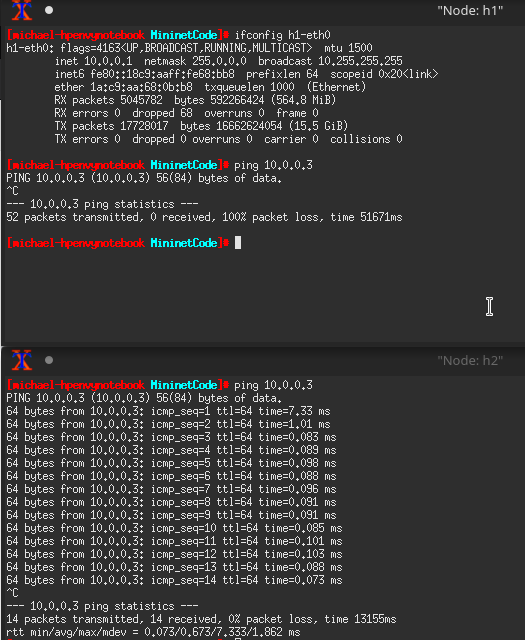
\includegraphics[width=0.8\textwidth]{images/icmpBlockDos}
	\caption{NACL Blocking traffic from the attacking node h1}
	\label{fig:images-icmpBlockDos}
\end{figure}

\subsection{Distributed Denial of Service}

The Distributed Denial of Service topology was verified within the Floodlight
web server. Figure \ref{fig:images-flDDoS} displays the results of this, with
8 switches with 8 hosts each, and a final switch connected to the single target
server node.

\begin{figure}[H]
	\centering
	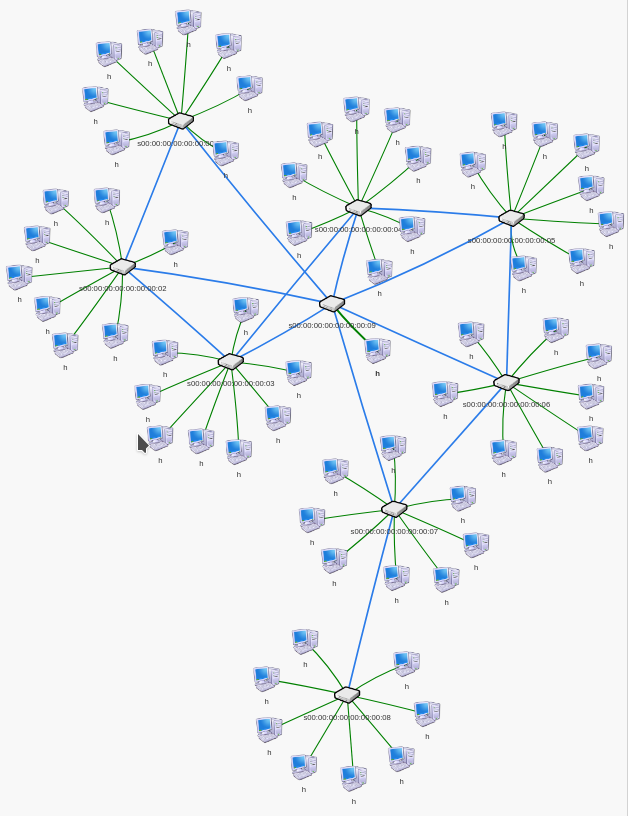
\includegraphics[width=0.8\textwidth]{images/flDDoS}
	\caption{Distributed Denial of Service Floodlight Topology}
	\label{fig:images-flDDoS}
\end{figure}

\subsubsection{SYN Flood}

The Wireshark packet capture tool is run on the server node. The filter option
used to capture only the incoming SYN packets from the attacking nodes is
'tcp.flag.syn== 1'. This results in the packet capture in Figure
\ref{fig:images-synFloodDDoSWs}. As with the Denial of Service attack, the "SYN"
flag can be seen in the packet information in the bottom of the window.

\begin{figure}[H]
	\centering
	\includegraphics[width=0.8\textwidth]{images/synFloodDDoSWS}
	\caption{Distributed Denial of Service SYN Flood Captured Packets}
	\label{fig:images-synFloodDDoSWs}
\end{figure}

The SYN flood was initiated much like that of the Denial of Service attack,
however, in this case, the commands were input via the Mininet CLI. The commands
took the following form:

\begin{lstlisting}[language=bash, caption=Mininet CLI commands for SYN DDoS Attack]
	<Host Name> hping --flood -S --rand-source <Target Name> &
\end{lstlisting}

In total, 28 hosts were used to launch the DDoS attack. The commands used can be
seen below in Figure \ref{fig:images-synFloodDDoSCli}.

\begin{figure}[H]
	\centering
	\includegraphics[width=0.8\textwidth]{images/synFloodDDoSCli}
	\caption{Mininet CLI command for SYN DDoS Attack}
	\label{fig:images-synFloodDDoSCli}
\end{figure}

Once the flooding attack has been running for a period of time, the curl command
is used on the user host node, which in this case was arbitrarily chosen as
"h65". The response of this command was repeated timeout errors, which can be
seen in Figure \ref{fig:images-synFloodDDoSCurl}, and confirms that a denial of
service has occurred.

\begin{figure}[H]
	\centering
	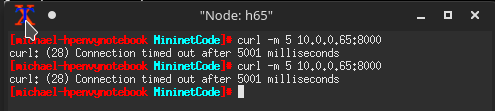
\includegraphics[width=0.8\textwidth]{images/synFloodDDoSCurl}
	\caption{Curl timeout due to the exhausted server resources}
	\label{fig:images-synFloodDDoSCurl}
\end{figure}

\subsubsection{ICMP Flood}

The Wireshark packet capture tool is run on the server node. The filter option
used to capture only the incoming ICMP packets from the attacking nodes is
'icmp'. This results in the packet capture in Figure
\ref{fig:images-icmpFloodDDoSWs}.

\begin{figure}[H]
	\centering
	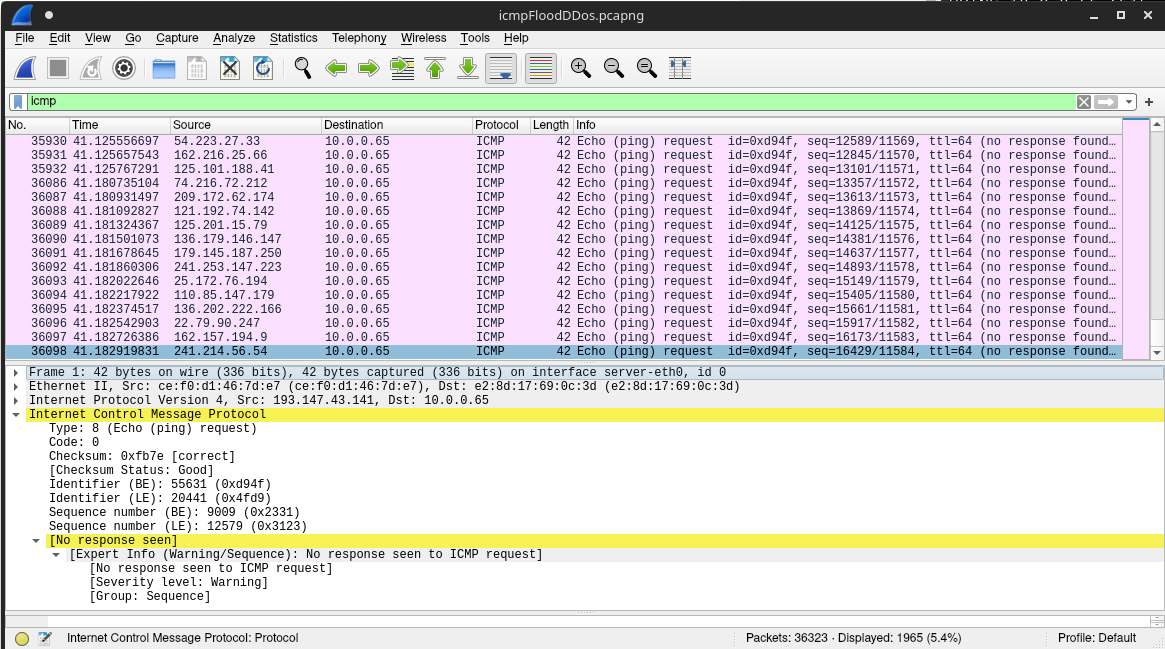
\includegraphics[width=0.8\textwidth]{images/icmpFloodDDoSWs}
	\caption{Distributed Denial of Service ICMP Flood Captured Packets}
	\label{fig:images-icmpFloodDDoSWs}
\end{figure}

The ICMP flood was initiated much like that of the previously described SYN
flood, however, in this case, the "-1" flag is used to specify that ICMP packets
must be sent. The commands took the following form:

\begin{lstlisting}[language=bash, caption=Mininet CLI commands for ICMP DDoS Attack]
	<Host Name> hping --flood -1 --rand-source <Target Name> &
\end{lstlisting}

In total, 28 hosts were used to launch the DDoS attack. The commands used can be
seen below in Figure \ref{fig:images-icmpFloodDDoSCli2}.

\begin{figure}[H]
	\centering
	\includegraphics[width=0.8\textwidth]{images/icmpFloodDDoSCli2}
	\caption{Mininet CLI command for ICMP DDoS Attack}
	\label{fig:images-icmpFloodDDoSCli2}
\end{figure}

Once the flooding attack has been running for a period of time, the ping command
is used on the user host node, which in this case was arbitrarily chosen as
"h65". The response of this command was repeated timeout errors, which can be
seen in Figure \ref{fig:images-icmpFloodDDoSCli}, and confirms that a denial of
service has occurred.

\begin{figure}[H]
	\centering
	\includegraphics[width=0.8\textwidth]{images/icmpFloodDDoSCli}
	\caption{Ping timeout due to the exhausted server resources}
	\label{fig:images-icmpFloodDDoSCli}
\end{figure}

As mentioned in Section 4, no mitigation techniques were introduced during this
stage of the simulation.
